% aspectratio : 169 for 16:9, 43 for 4:3, default 3:2
% nobackgroundmain: removes TU Wien ICT style in non-title slides
% nobackgroundfirst: remove TU Wien background in title and last slide
\documentclass[aspectratio=169, nobackgroundmain]{beamer}

\mode<presentation>
{
 % noauthor, notitle, nocircle, noframenumber hide foot line elements
 % reversetitle: blue background and white text for slide titles, otherwise blue text and white background
 % logoleft, logocenter, logoright: set logos in title slide. Default: left TU, right ICT
 % backgroundfirst, backgroundmain define slide backgrounds
 \usetheme[reversetitle, noauthor]{Wien} 
}       

\usepackage[utf8]{inputenc}
\usepackage[absolute,overlay]{textpos}
\usepackage{url}
\usepackage{verbatim}  % inline code (\verb||)
\usepackage{listings}
\usepackage{siunitx}  % easy handling of value + unit (e.g. \SI{10}{\pF})
\usepackage{booktabs}  % nicer tables (e.g. \toprule)

\usepackage{graphicx}
\graphicspath{{./}{./figures/}}  
\usepackage{appendixnumberbeamer}

\usepackage{csquotes} % removes biber warning
\usepackage[  % ieee style citations (e.g. [1])
	backend     = biber,
	maxbibnames = 99,
	autocite    = footnote,
	style	      = ieee,
	citestyle   = numeric-comp,
	doi=false, isbn=false
]{biblatex}
\addbibresource{bibliography/bibliography.bib}

\usepackage[nobiblatex]{xurl}  % line breaks in URLs

% To avoid a warning from the hyperref package:
\pdfstringdefDisableCommands{%
  \def\translate{}%
}

\lstset{
  language=bash,
  basicstyle=\ttfamily
}

% add missing hyphenations
\hyphenation{im-ple-men-ta-tions}

\renewcommand*{\bibfont}{\footnotesize}

%%%%%%%%%%%%%%%%%%%%%%%%%%%%%%%%%%%%%%%%%%%%%%%%%%%%%%%%%%%%%%%%%%%%%%%%%%%%%

\title{Integration of an Encryption Accelerator
into an Open-Source Low-Power Microcontroller}

\subtitle{384.178 SoC Design Lab}

\author[Severin Jäger]{Severin Jäger}
   
\date{March 8, 2022}

\begin{document}

\begin{frame}
  \titlepage
\end{frame}

%%%%%%%%%%%%%%%%%%%%%%%%%%%%%%%%%%%%%%%%%%%%%%%%%%%%%%%%%%%%%%%%%%%%%%%%%%%%% 
%%%%%%%%%%%%%%%%%%%%%%%%%%%%%%%%%%%%%%%%%%%%%%%%%%%%%%%%%%%%%%%%%%%%%%%%%%%%%

%%%%%%%%%%%%%%%%%%%%%%%%%%%%%%%%%%%%%%%%%%%%%%%%%%%%%%%
\begin{frame}[fragile]{Motivation}
  \begin{itemize}
    \item Increasing demand for near-sensor processing (signal processing, simple machine learning)
    \item Highly energy-constrained edge devices
    \item Privacy crucial for certain applications (e.g. biomedical devices, surveillance, home automation)
    \item Open source as gold standard for security - why not in hardware?
\end{itemize}

\begin{block}{}
    \centering
   Goal: Provide energy-efficient cryptographic support for an open-source low-power microcontrollers
\end{block}
\end{frame}

%%%%%%%%%%%%%%%%%%%%%%%%%%%%%%%%%%%%%%%%%%%%%%%%%%%%%%%
\begin{frame}[fragile]{Recap I: Setup}
  \begin{columns}
      \begin{column}{0.5\textwidth}
          \begin{itemize}
              \item PULPissimo SoC [1]: Single-core microcontroller with full set of peripherals
              \item Open hardware (ISA, RTL)
              \item Focused on energy efficiency, not performance
              \item Hardware processing engine (HWPE) allows accelerator integration
          \end{itemize}
      \end{column}
      \begin{column}{0.49\textwidth}
          \begin{figure}
              \raggedleft
              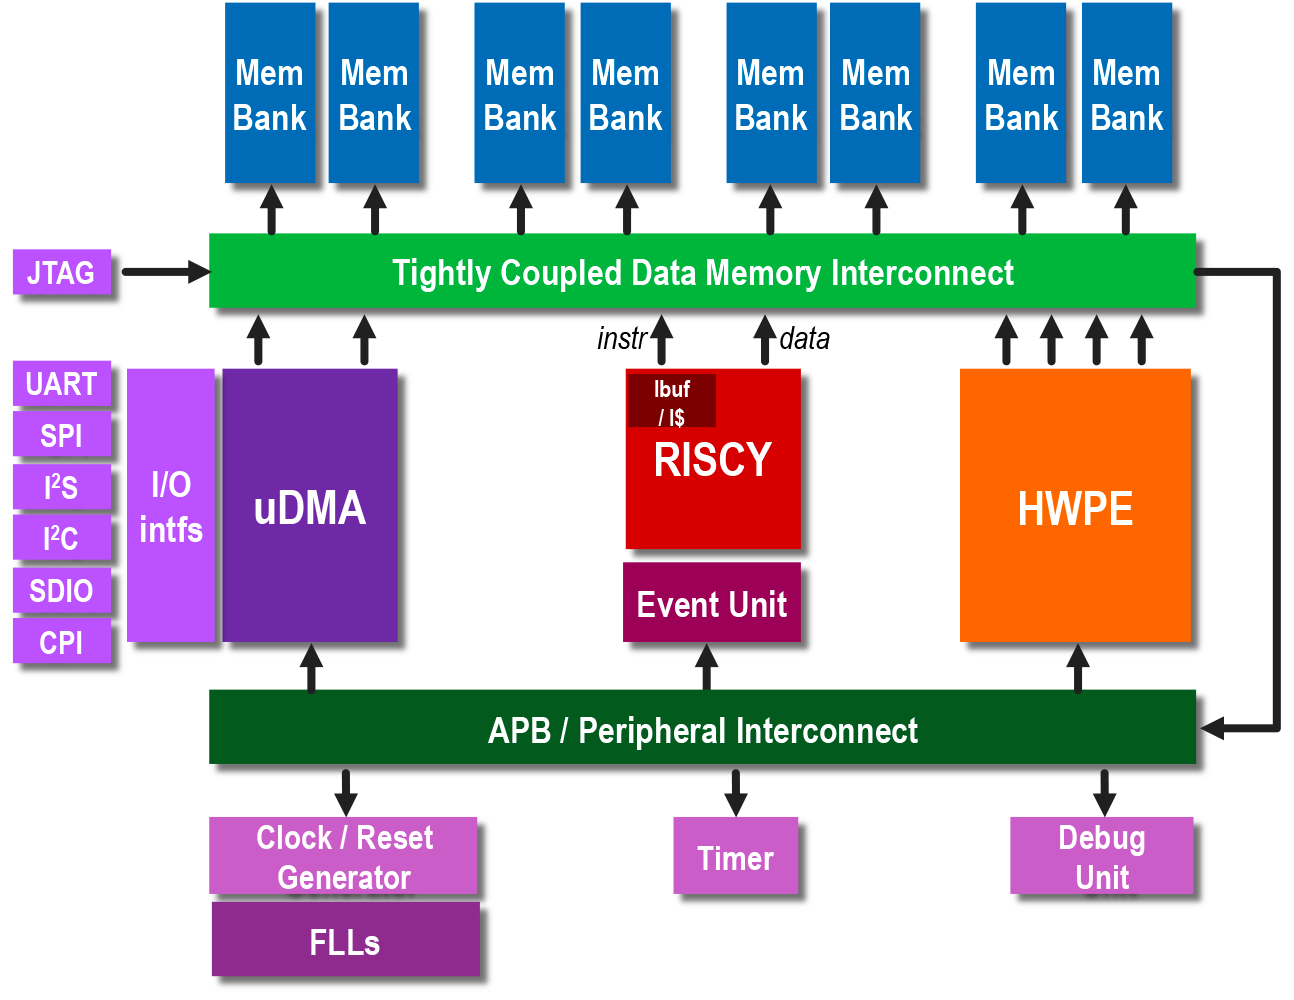
\includegraphics[width=1\textwidth]{pulpissimo_arch.png}
          \end{figure}
      \end{column}
  \end{columns}
\end{frame}

%%%%%%%%%%%%%%%%%%%%%%%%%%%%%%%%%%%%%%%%%%%%%%%%%%%%%%%
\begin{frame}[fragile]{Pulp Hardware Processing Engine (HWPE)}
  \begin{columns}
      \begin{column}{0.5\textwidth}
          \begin{itemize}
          \item Data exchange via shared L2 memory (no DMA or the like required)
          \item Control flow defined via peripheral interconnect (memory-mapped)
          \item Pointers and parameters exchanged, then autonomous operation
          \item Can be integrated into PULPissimo as well as larger clusters in the PULP ecosystem
          \item Template available open source
      \end{itemize}
      \end{column}
      \begin{column}{0.49\textwidth}
          \begin{figure}
              \raggedleft
              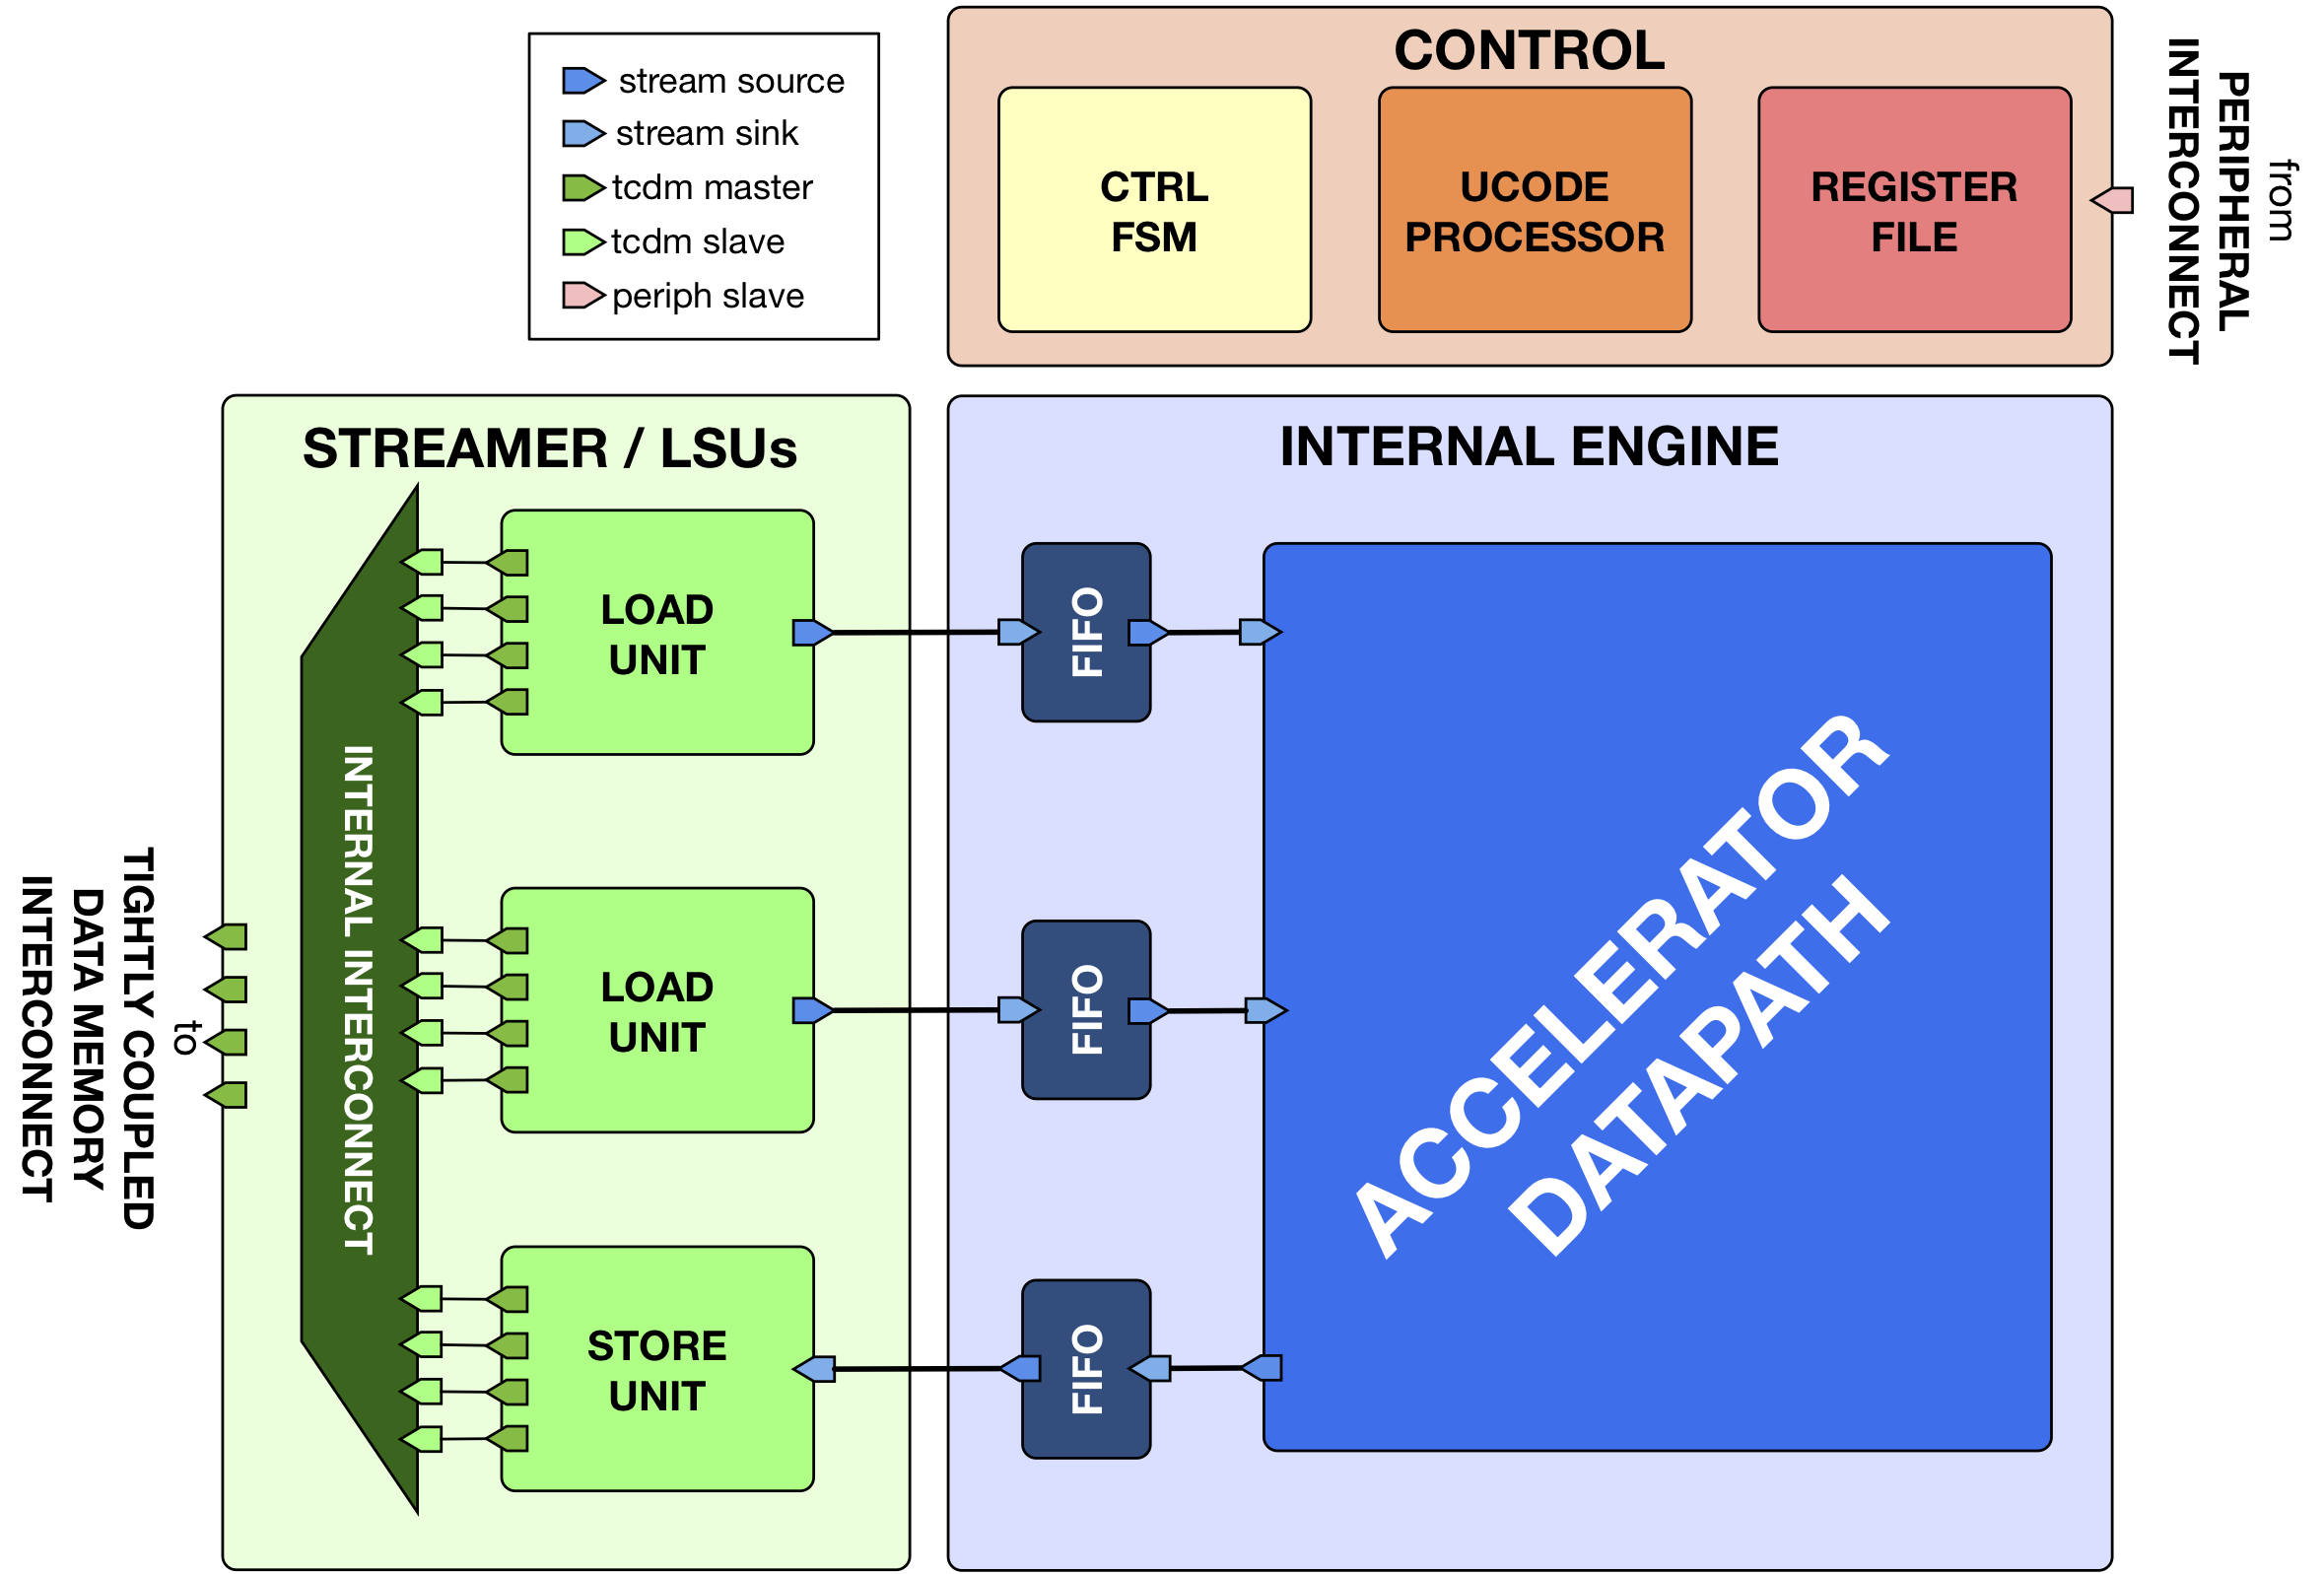
\includegraphics[width=1\textwidth]{hwpe.png}
          \end{figure}
      \end{column}
  \end{columns}
\end{frame}

%%%%%%%%%%%%%%%%%%%%%%%%%%%%%%%%%%%%%%%%%%%%%%%%%%%%%%%
\begin{frame}[fragile]{Project Goal}
  \begin{itemize}
    \item Implement an AES HWPE \begin{itemize}
      \item Encryption only
      \item 128 bit keys
      \item Only straightforward electronic code book (ECB) mode \begin{itemize}
        \item This is not state of the art!
      \end{itemize}
    \end{itemize} 
    \item Compare to reference software
\end{itemize}

\begin{block}{}
    \centering
   What can be gained from implementing AES in hardware?
\end{block}
\end{frame}

%%%%%%%%%%%%%%%%%%%%%%%%%%%%%%%%%%%%%%%%%%%%%%%%%%%%%%%
\begin{frame}[fragile]{Reference Software Implementation}

  \begin{itemize}
      \item Software reference implementation to assess gains
      \item \verb|tiny-AES-c| available open source [2]
      \item Lightweight and portable C implementation
      \item Code size \SI{2.1}{kB} (compiled for PULPissimo)
      \item Extremely simple API (\verb|AES_init_ctx()|, \verb|AES_ECB_encrypt()| sufficient)
      \item Simple demo application encrypting $N$ words \& checking results
  \end{itemize}
  
\end{frame}

%%%%%%%%%%%%%%%%%%%%%%%%%%%%%%%%%%%%%%%%%%%%%%%%%%%%%%%%%%%%%%%%%%%%%%%%%%%%%
\begin{frame}[fragile]{Verilog AES IP cores}

\small
  \begin{table}[h]
    \centering
    \begin{tabular}{c|c c c}
        \toprule
        Core &  \verb|tiny_aes| & \verb|aes_128| [3] & \verb|secworks_aes| \\
        \midrule
        Cycles/Op &  1 & 12 & 4\\
        Latency (cylces) & 21 & 12 & 14\\
        LUTs & 4588 & 487 & 3327 \\
        Registers & 4474 & 402 & 2990 \\
        BRAM Tiles & 68 & 5 & 0 \\
        Max. Frequency [MHz] & 375.9 & 180.5 & 124.8 \\
        Decryption & no & no  & yes \\
        AES 256 & no & no & yes\\
        \bottomrule
    \end{tabular}
\end{table}

\centering
\footnotesize
Resource consumption and clock frequency on Nexys4DDR with Vivado 2020.2
\normalsize

\begin{block}{}
  \centering
  \verb|aes_128| selected due to minimal resource consumption and sufficient performance
\end{block}

\end{frame}

%%%%%%%%%%%%%%%%%%%%%%%%%%%%%%%%%%%%%%%%%%%%%%%%%%%%%%%
\begin{frame}[fragile]{HWPE Operation}
  \begin{columns}
    \begin{column}{0.5\textwidth}
      \begin{itemize}
        \item Input data written to shared memory by CPU
        \item Control registers set by CPU (from software) \begin{itemize}
          \item Source and destination pointers
          \item Number of bytes to be loaded
          \item Start operation
        \end{itemize}
        \item HWPE FSM controls data ports and data path (interleaving): \begin{itemize}
          \item Stream of input words fetched from shared memory
          \item Data path computation (AES)
          \item Stream of output words written to shared memory
        \end{itemize}
    \end{itemize}
    \end{column}
    \begin{column}{0.49\textwidth}
        \begin{figure}
            \raggedleft
            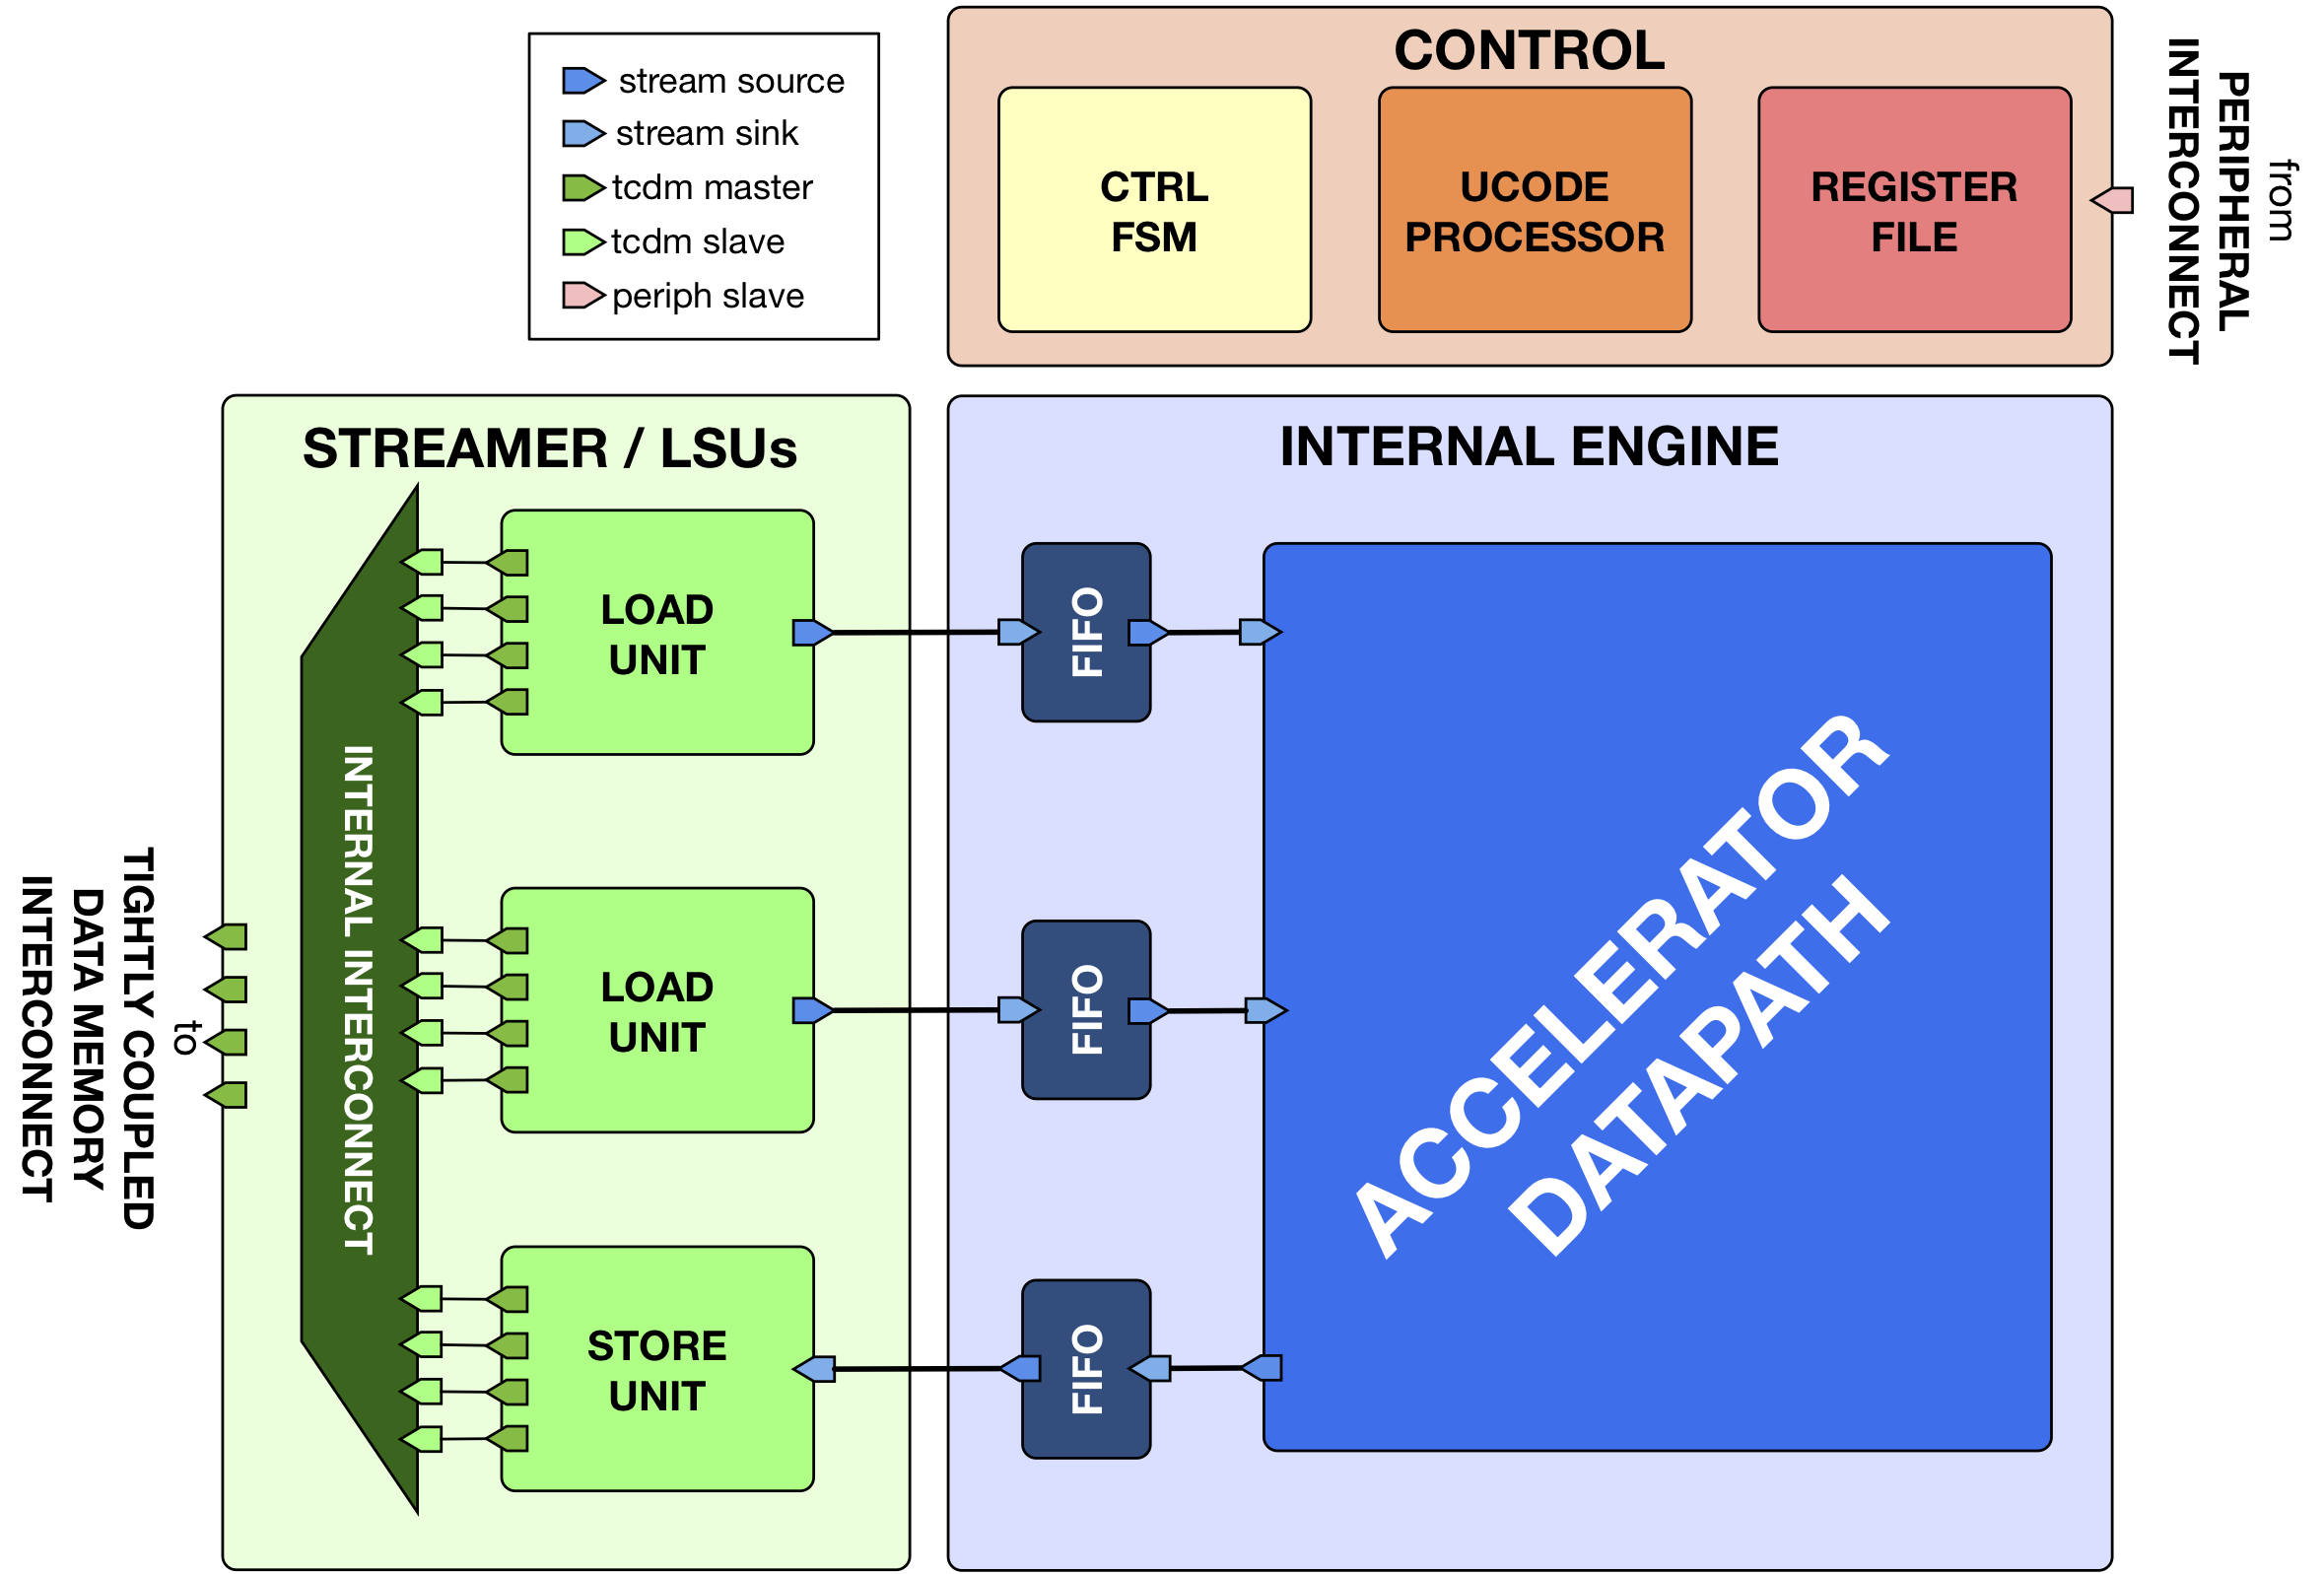
\includegraphics[width=1\textwidth]{hwpe.png}
        \end{figure}
    \end{column}
  \end{columns} 
\end{frame}

%%%%%%%%%%%%%%%%%%%%%%%%%%%%%%%%%%%%%%%%%%%%%%%%%%%%%%%
\begin{frame}[fragile]{HWPE Datapath}

  \begin{itemize}
      \item Based on HWPE MAC example
      \item 32 bit wide memory interfaces
      \item (Un-)stackers for 128 bit AES words
      \item Pipelined operation
      \item Ready/valid handshake between all stages (forward \& backward dependencies)
  \end{itemize}
  
  \begin{figure}
    \raggedleft
    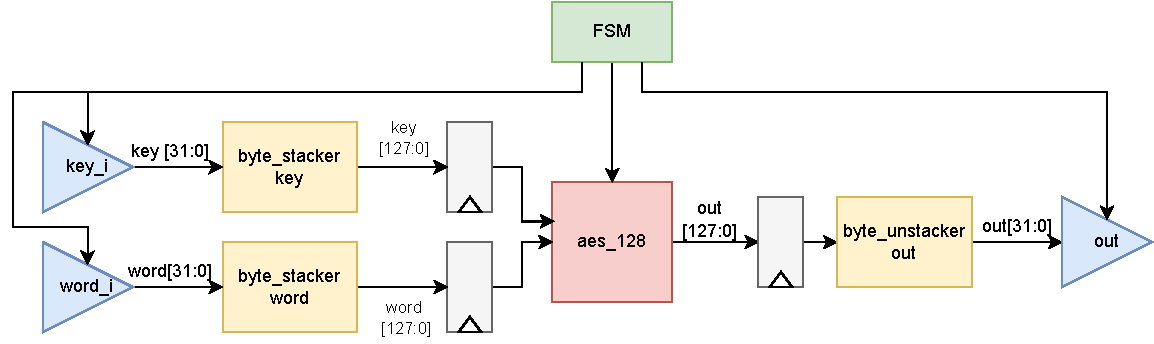
\includegraphics[width=0.9\textwidth]{hwpe_aes.pdf}
\end{figure}
  
\end{frame}

%%%%%%%%%%%%%%%%%%%%%%%%%%%%%%%%%%%%%%%%%%%%%%%%%%%%%%%
\begin{frame}[fragile]{HWPE Software}

  \begin{itemize}
      \item Utilising device driver from HWPE MAC example
      \item Write test data ($N \times 128$ bit keys and words) to memory
      \item Define HWPE registers \begin{itemize}
        \item Bytecode defining operation
        \item Source and destination pointers
        \item Number of bytes to be loaded and stored
      \end{itemize}
      \item Start HWPE operation (via register)
      \item Wait for HPWE done event
      \item Validate results
  \end{itemize}  
\end{frame}

%%%%%%%%%%%%%%%%%%%%%%%%%%%%%%%%%%%%%%%%%%%%%%%%%%%%%%%
\begin{frame}[fragile]{Results}
  \begin{table}[h]
    \centering
    \begin{tabular}{c|c c}
        \toprule
         &  AES Software & AES HWPE  \\
        \midrule
        Runtime $N=32$ & \SI{2876}{\mu s} & \SI{10}{\mu s} \\
        Relative speed-up & 1 & 287.6 \\
        Runtime further encryption & \SI{61}{\mu s} & \SI{280}{ns} \\
        Code size & 9816 bytes & 9140 bytes\\
        \bottomrule
    \end{tabular}
  \end{table}

  \begin{block}{}
     \begin{itemize}
       \item Greatly reduced runtime leads to more CPU sleep time $\implies$ energy savings
       \item Code size reduced
       \item No area estimation due to synthesis issues
     \end{itemize}
  \end{block}
\end{frame}

%%%%%%%%%%%%%%%%%%%%%%%%%%%%%%%%%%%%%%%%%%%%%%%%%%%%%%%
\begin{frame}[fragile]{Challenges I}
  \begin{itemize}
      \item Simulator (QuestaSim) only available on ICT EDA server \begin{itemize}
        \item Nasty setup including several bash scripts
        \item Slow VPN connection $\implies$ terribly slow mounted file system
      \end{itemize}
      \item PULPissimo is a \textbf{huge} design $\implies$ long build \& simulation times, hard debugging \begin{itemize}
        \item Hardware change to vcd takes at least 10 minutes
        \item vcd file sizes are quickly 10 GB
      \end{itemize}
      \item PULP is an academic project $\implies$ little documentation
  \end{itemize}

  \begin{columns}
    \begin{column}{0.22\textwidth}
      \begin{figure}
        \centering
        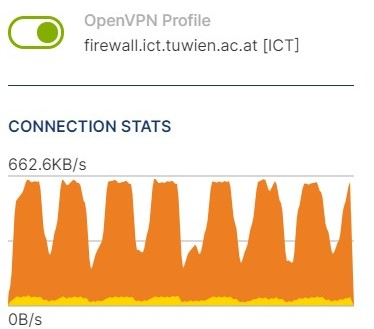
\includegraphics[width=\textwidth]{vpn.jpeg}
      \end{figure}
    \end{column}
    \begin{column}{0.78\textwidth}
      \begin{figure}
        \centering
        
\includegraphics[width=0.5\textwidth]{loading.png}
        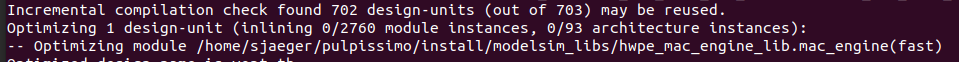
\includegraphics[width=0.8\textwidth]{modules.png}
        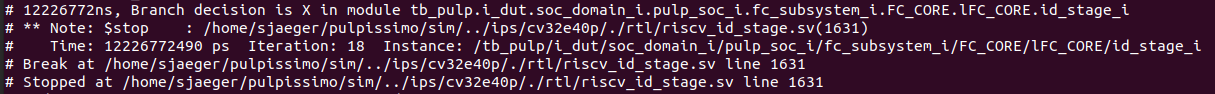
\includegraphics[width=1\textwidth]{branch-x.png}
      \end{figure}
    \end{column}
  \end{columns}
\end{frame}

%%%%%%%%%%%%%%%%%%%%%%%%%%%%%%%%%%%%%%%%%%%%%%%%%%%%%%%
\begin{frame}[fragile]{Challenges II}

  \begin{itemize}
      \item Errors are normal (e.g. due to different QuestaSim version)
      \item HWPE template is extremely powerful (620 bit control signal) $\implies$ hard to understand and modify \begin{itemize}
        \item Solution: Leave control logic as it is, find suitable software configuration
      \end{itemize}
      \item AES HWPE is faster than PULPissimo timer resolution $\implies$ runtimes from vcd
      \item Provided scripts do not like me
  \end{itemize}

  \begin{columns}
    \begin{column}{0.5\textwidth}
      \begin{figure}
        \centering
        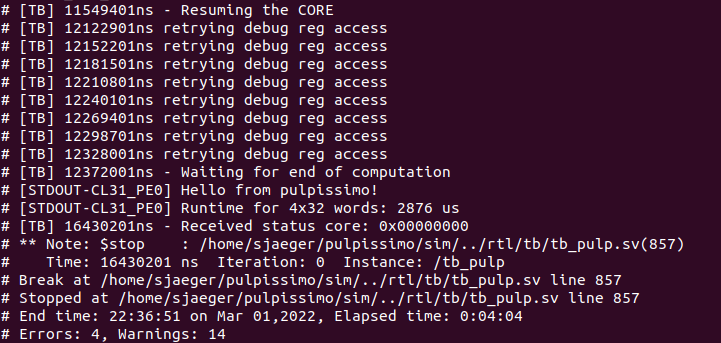
\includegraphics[width=0.9\textwidth]{vsim.png}
      \end{figure}
    \end{column}
    \begin{column}{0.5\textwidth}
      \begin{figure}
        \centering
        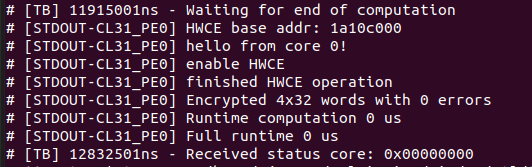
\includegraphics[width=0.8\textwidth]{runtime.png}
        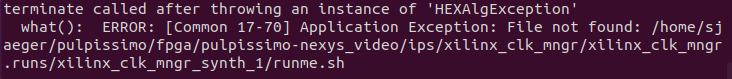
\includegraphics[width=\textwidth]{vivado.png}
      \end{figure}
    \end{column}
  \end{columns}
  \begin{figure}
    \centering
    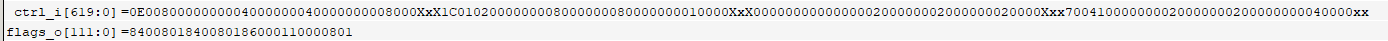
\includegraphics[width=\textwidth]{ctrl_flags.png}
  \end{figure}
\end{frame}

%%%%%%%%%%%%%%%%%%%%%%%%%%%%%%%%%%%%%%%%%%%%%%%%%%%%%%%
\begin{frame}[fragile]{Summary and Outlook}

  \begin{itemize}
      \item AES HPWE integrated into PULPissimo \begin{itemize}
        \item Speed-up of 287.6 achieved
        \item Code size reduced
        \item Likely significant energy savings
      \end{itemize}
  \end{itemize}  

  \begin{itemize}
    \item Possible extensions \begin{itemize}
      \item Investigate different AES implementations or other algorithms
      \item ASIC implementation of HWPE to analyse area and power
    \end{itemize}
\end{itemize}  
\end{frame}


%%%%%%%%%%%%%%%%%%%%%%%%%%%%%%%%%%%%%%%%%
\begin{frame}[fragile]{References}
  \fontsize{11pt}{10}\selectfont
    \begin{tabular}{p{1cm}p{12cm}}
      {[1]} & PULPissimo repository on GitHub \url{https://github.com/pulp-platform/pulpissimo} \\
      {[2]} & \verb|tiny-AES-c| repository on GitHub \url{https://github.com/kokke/tiny-AES-c} \\
      {[3]} & \verb|aes_128| repository on GitHub \url{https://github.com/www-asics-ws/aes_128}\\
    \end{tabular}
  \end{frame}


%%%%%%%%%%%%%%%%%%%%%%%%%%%%%%%%%%%%%%%%%%%%%%%%%%%%%%%%%%%%%%%%%%%%%%%%%%%%% 
%%%%%%%%%%%%%%%%%%%%%%%%%%%%%%%%%%%%%%%%%%%%%%%%%%%%%%%%%%%%%%%%%%%%%%%%%%%%%

\end{document}
